\documentclass[11pt,a4paper]{article}
\usepackage[utf8]{inputenc}
\usepackage[french]{babel}
\usepackage[T1]{fontenc}
\usepackage{amsmath}
\usepackage{amsfonts}
\usepackage{amssymb}
\usepackage{graphicx}
\usepackage{listings}
\usepackage{float}
\usepackage{xcolor,times}

\newcommand*\styleC{\fontsize{9}{10pt}\usefont{T1}{ptm}{m}{n}\selectfont }
\newcommand*\styleD{\fontsize{9}{10pt}\usefont{OT1}{pag}{m}{n}\selectfont }

\makeatletter
% on fixe le langage utilisé
\lstset{language=matlab}
\edef\Motscle{emph={\lst@keywords}}
\expandafter\lstset\expandafter{%
  \Motscle}
\makeatother


\definecolor{Ggris}{rgb}{0.45,0.48,0.45}

\lstset{emphstyle=\rmfamily\color{blue}, % les mots réservés de matlab en bleu
basicstyle=\styleC,
keywordstyle=\ttfamily,
commentstyle=\color{green}\styleC, % commentaire en gris
numberstyle=\tiny\color{red},
numbers=left,
numbersep=10pt,
lineskip=0.7pt,
showstringspaces=false}
%  % inclure le fichier source
\newcommand{\FSource}[1]{%
\lstinputlisting[texcl=true]{#1}
}

%%%%%%%%%
\textwidth=15cm
\textheight=21cm
%\hoffset=-2.5cm
\tolerance=9000
\hbadness=9000
\pretolerance=2500


\author{Sacha GRELET-RIOUT et Hugo BRUHIER}
\title{TD/Mini-projet\\Classification bayésienne\\ \normalsize Image 3 : De l'image à l'information\\Reconnaissance de formes\\\emph{Télécom Saint-Étienne}}
\date{}



\begin{document}
\maketitle

%\tableofcontents
%\noindent\hrulefill

\section{Introduction}

Nous allons, lors de ce TD, travailler sur la classification bayésienne et faire l'application des formules  et principes vus en cours sur des cas pratiques sur \emph{MatLab}. Pour bien poser certaines notations on a :
\begin{equation}
p(w_i|x) = \frac{p(x|w_i)\mathbb{P}(w_i)}{p(x)}
\end{equation}
avec :
\begin{itemize}
\item $p(w_i|x)$ la probabilité à postériori,
\item $p(x|w_i)$ la vraisemblance,
\item $\mathbb{P}(w_i)$ la probabilité à priori,
\item $p(x)$ la probabilité totale.
\end{itemize}
On dispose de la formule suivante\footnote{Vraie dans le cas d'un problème à deux classes.} qui nous permettra de faire des calculs plus tard dans le code :
\begin{equation}
p(x) = p(x|w_1)\mathbb{P}(w_1) + p(x|w_2)\mathbb{P}(w_2)
\end{equation}


\section{Exercice 1 : Décision bayésienne}

Ici on regarde un problème à deux classes que l'on va modéliser par deux lois gaussiennes, la variance $\sigma^2$ sera la même et les moyennes respectives seront 0 et 1 :

\begin{equation}
p(x|w_1) = \frac{1}{\sqrt{\pi}}\,\text{exp}\left[-x^2\right]
\end{equation}

\begin{equation}
p(x|w_2) = \frac{1}{\sqrt{\pi}}\,\text{exp}\left[-(x-1)^2\right]
\end{equation}

On cherche ici à déterminer la valeur de la variance $\sigma^2$, pour cela on rappelle la formule d'une loi normale de paramètres $\mu$ et $\sigma$ :
$$
\mathcal{N}(\mu,\sigma) = \frac{1}{\sqrt{2\sigma^2\pi}}\,\text{exp}\left[-\frac{(x-\mu)^2}{2\sigma^2}\right]
$$
On procède à l'identification suivante :
\begin{align*}
2 \sigma^2 &= 1 \\
\Leftrightarrow \sigma^2 &= \frac{1}{2} \\
\Leftrightarrow \sigma &= \frac{1}{\sqrt{2}}
\end{align*}

Dans un premier temps nous allons prendre l'équiprobabilité comme probabilités à priori, donc nous avons :
$$
\left \{
\begin{array}{c @{\,\,\,=\,\,\,} c}
    \mathbb{P}(w_1) & 0,5\\
    \mathbb{P}(w_2) & 0,5
\end{array}
\right.
$$
Traçons sur la figure \ref{fig.exo1_graph1} les densités de probabilité des deux classes, les probabilités à postériori ainsi que le seuil bayésien.

\begin{figure}[H]
\center
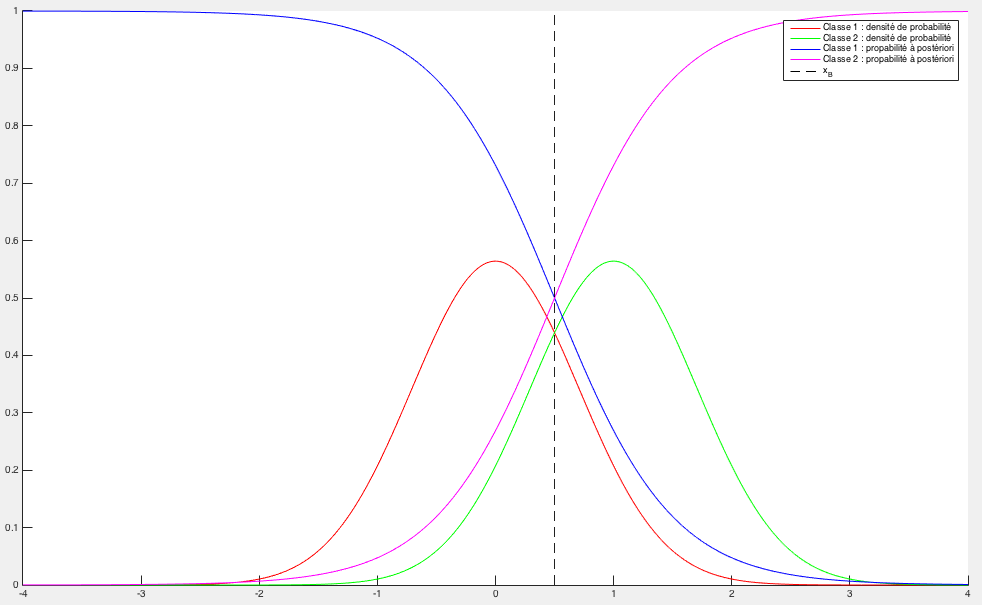
\includegraphics[width=15cm]{exo1_graph1.png}
\label{fig.exo1_graph1}
\caption{Données de probabilités dans le cas initial}
\end{figure}

Nous cherchons le seuil de classification, tout d'abord nous allons le trouver en déroulant de manière littérale les calculs puis nous allons coder sa recherche pour vérifier expérimentalement le résultat. On définit le seuil $x_B$ par :
\begin{equation}
g_1(x_B) = \text{log}\left[p(x_B|w_1)\mathbb{P}(w_1)\right] = g_2(x_B)
\label{eq.def.seuil.bay}
\end{equation}
On cherche donc $x$ tel que l'égalité suivante soit vérifiée :
$$
\text{log}\left[p(x|w_1)\mathbb{P}(w_1)\right] = \text{log}\left[p(x|w_2)\mathbb{P}(w_2)\right]
$$
On remplace $p(x|w_1)$ et $p(x|w_2)$ par leurs expressions respectives :
$$
\text{log}\left[\frac{1}{\sqrt{\pi}}\,\text{exp}\left[-x^2\right]\mathbb{P}(w_1)\right] = \text{log}\left[\frac{1}{\sqrt{\pi}}\,\text{exp}\left[-(x-1)^2\right]\mathbb{P}(w_2)\right]
$$
On utilise une propriété bien connue du logarithme\footnote{$\text{log}(x.y) = \text{log}(x) + \text{log}(y)$} pour séparer les termes :
$$
\text{log}\left[\frac{1}{\sqrt{\pi}}\right] + \text{log}\left[\text{exp}\left[-x^2\right]\right] + \text{log}\left[\mathbb{P}(w_1)\right] = \text{log}\left[\frac{1}{\sqrt{\pi}}\right] + \text{log}\left[\text{exp}\left[-(x-1)^2\right]\right] + \text{log}\left[\mathbb{P}(w_2)\right]
$$
Avec l'égalité $\mathbb{P}(w_1) = \mathbb{P}(w_1)$ on peut simplifier aisément notre expression :
$$
\text{log}\left[\text{exp}\left[-x^2\right]\right] = \text{log}\left[\text{exp}\left[-(x-1)^2\right]\right]
$$
Les fonctions log et exp sont réciproques l'une à l'autre, on simplifie donc par :
$$
-x^2 = -(x-1)^2
$$
On développe le second terme de l'expression :
\begin{align*}
-x^2 &= -x^2 + 2x - 1 \\
\Leftrightarrow x &= 0,5
\end{align*}
On trouve donc notre seuil bayésien :
$$
x_B = 0,5
$$

En utilisant le code ci-dessous on recherche expérimentalement cette valeur du seuil bayésien. On trouve bien en sortie une valeur de seuil de $0,5$.

\noindent\hrulefill
\begin{lstlisting}[language=matlab]
i = 1;
g1 = log(pxw1(1) * Pw1);
g2 = log(pxw2(1) * Pw2);
for k = 2 : length(x)
    g1m = log(pxw1(k) * Pw1);
    g2m = log(pxw2(k) * Pw2);
    
    if (g1 - g2)*(g1m - g2m) < 0
        xB(i) = x(k);
        i = i + 1;
    end
    
    g1 = log(pxw1(k) * Pw1);
    g2 = log(pxw2(k) * Pw2);
    
end
\end{lstlisting}
\noindent\hrulefill


On recherche maintenant à quantifier la probabilité de l'erreur. On rappelle la formule de cette probabilité dans le cas à deux régions :
\begin{equation}
\mathbb{P}(\text{erreur}) = \int_{\mathcal{R}_2}p(x|w_1)\mathbb{P}(w_1)dx + \int_{\mathcal{R}_1}p(x|w_2)\mathbb{P}(w_2)dx
\end{equation}
En utilisant notre seuil $x_B$ on peut réécrire l'erreur comme :
$$
\mathbb{P}(\text{erreur}) = \int_{x_B}^{+\infty}p(x|w_1)\mathbb{P}(w_1)dx + \int_{-\infty}^{x_B}p(x|w_2)\mathbb{P}(w_2)dx
$$
On va calculer les intégrales par la méthode des rectangles via la portion de code suivante :

\noindent\hrulefill
\begin{lstlisting}[language=matlab]
indices = find(x <= xB);
M = length(indices);
Perreur = Pas * sum(pxw2(indices) * Pw2);
Perreur = Perreur + Pas * sum(pxw1(indices(M) + 1:L) * Pw1);
\end{lstlisting}
\noindent\hrulefill

On trouve avec la bonne valeur du seuil une probabilité d'erreur de $0,2398$. On trace sur la figure  la probabilité d'erreur en fonction de la position du seuil $x_B$, on voit que pour d'autres valeurs du seuil que celle que l'on a trouvé la probabilité de faire une erreur augmente.

Nous allons maintenant changer les probabilités à priori pour nous placer dans un cas non-équi-probable pour voir les changements que cela va apporter sur notre classifieur. Maintenant on a :
$$
\left \{
\begin{array}{c @{\,\,\,=\,\,\,} c}
    \mathbb{P}(w_1) & 0,9\\
    \mathbb{P}(w_2) & 0,1
\end{array}
\right.
$$

La figure suivante montre les même informations que la figure \ref{fig.exo1_graph1} avec les nouvelles probabilités à priori :

\begin{figure}[H]
\center
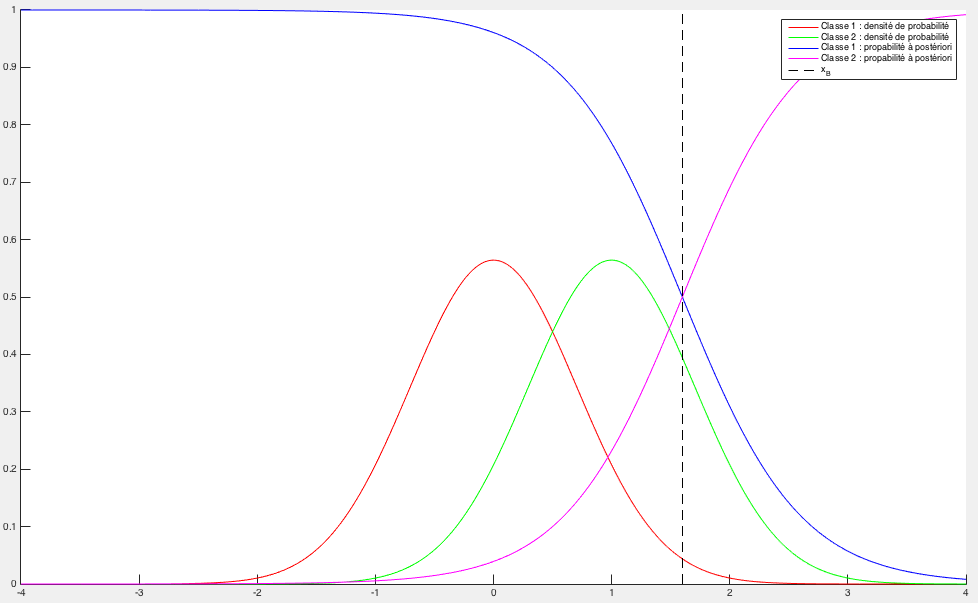
\includegraphics[width=15cm]{exo1_graph_nvProbas.png}
\label{fig.exo1_graph_nvProbas}
\caption{Données de probabilités dans le cas des nouvelles probabilités à priori}
\end{figure}


On réitère ici le calcul du seuil de décision bayésienne, définit à l'équation \ref{eq.def.seuil.bay} page \pageref{eq.def.seuil.bay}, on recherche donc $x$ tel que :
$$
\text{log}\left[p(x|w_1)\mathbb{P}(w_1)\right] = \text{log}\left[p(x|w_2)\mathbb{P}(w_2)\right]
$$
On remplace encore $p(x|w_1)$ et $p(x|w_2)$ par leurs expressions respectives :
$$
\text{log}\left[\frac{1}{\sqrt{\pi}}\,\text{exp}\left[-x^2\right]\mathbb{P}(w_1)\right] = \text{log}\left[\frac{1}{\sqrt{\pi}}\,\text{exp}\left[-(x-1)^2\right]\mathbb{P}(w_2)\right]
$$
On sépare les termes par la propriété du logarithme :
$$
\text{log}\left[\frac{1}{\sqrt{\pi}}\right] + \text{log}\left[\text{exp}\left[-x^2\right]\right] + \text{log}\left[\mathbb{P}(w_1)\right] = \text{log}\left[\frac{1}{\sqrt{\pi}}\right] + \text{log}\left[\text{exp}\left[-(x-1)^2\right]\right] + \text{log}\left[\mathbb{P}(w_2)\right]
$$
On simplifie :
$$
\text{log}\left[\text{exp}\left[-x^2\right]\right] + \text{log}\left[\mathbb{P}(w_1)\right] = \text{log}\left[\text{exp}\left[-(x-1)^2\right]\right] + \text{log}\left[\mathbb{P}(w_2)\right]
$$
On passe toutes les constantes du même côté et on simplifie les exponentielles via les logarithmes :
$$
-x^2 = -(x-1)^2 + \text{log}\left[\mathbb{P}(w_2)\right] - \text{log}\left[\mathbb{P}(w_1)\right]
$$
On développe l'expression pour supprimer les termes au carré :
$$
-x^2 = -x^2 + 2x - 1 + \text{log}\left[\frac{\mathbb{P}(w_2)}{\mathbb{P}(w_1)}\right]
$$
On modifie un peu l'expression en remplaçant $\mathbb{P}(w_1)$ et $\mathbb{P}(w_1)$ par leurs valeurs :
$$
2x =  1 - log\left(\frac{1}{9}\right)
$$
Ce qui nous donne :
$$
x_B \simeq 1,5986
$$

Le calcul dans le programme nous donne pour valeur expérimentale du seuil $1,6$ ce qui est cohérent\footnote{De plus nous utilisons un pas entre chaque valeur du vecteur $x$ de $0,01$ pour diminuer le temps de calcul et l'espace mémoire nécessaire.}.
\\ \\
On va ne pas prendre en compte le dénominateur dans le calcul des probabilités à postériori, cela nous donne la figure \ref{fig.exo1_graph_numerateur}. On constate que le seuil de classification bayésienne $x_B$ n'est pas modifié que l'on prenne en compte ou non la probabilité totale au dénominateur car cette quantité n'est pas discriminante dans la classification.

\begin{figure}[H]
\center
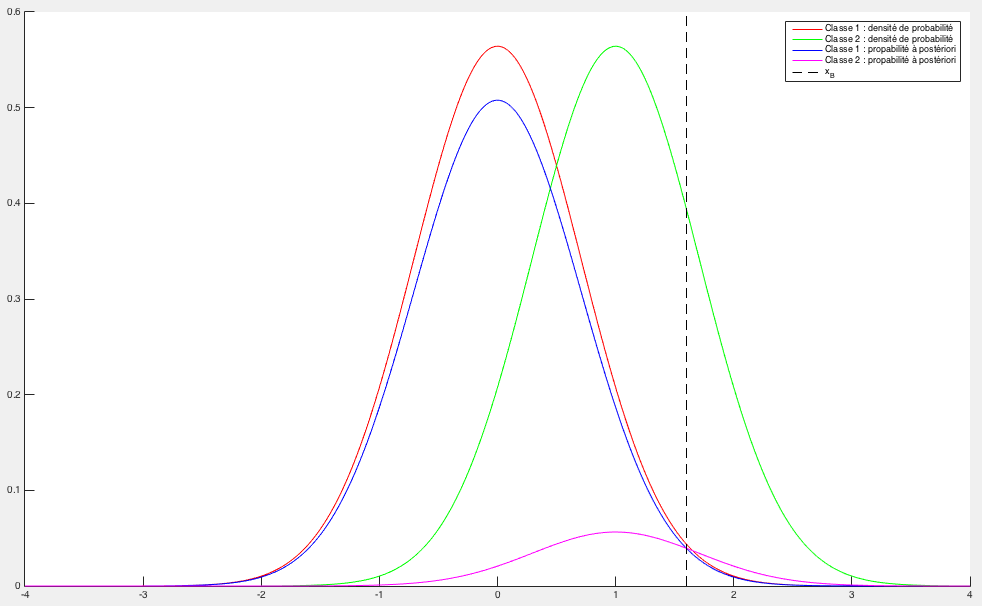
\includegraphics[width=15cm]{exo1_graph_numerateur.png}
\label{fig.exo1_graph_numerateur}
\caption{Données de probabilités sans le dénominateur}
\end{figure}

\section{Exercice 2 : Application à la détection de visages automatique}


\subsection{Partie I : Apprentissage du modèle de peau}

\subsubsection{Sélection des échantillons d'apprentissage}

On considère que le modèle de peau peut être modélisé par un modèle gaussien multi-varié. On pose $\textbf{x}$ le vecteur contenant les données de couleurs d'un pixel, si on pose $w_1$ le classe "peau" on écrit :
\begin{equation}
p(\textbf{x}|w_1) = \frac{1}{(2\pi)^{\frac{d}{2}}|\Sigma_1|^{\frac{1}{2}}}\,\text{exp}\left[-\frac{1}{2}(\textbf{x}-\mu_1)^T \Sigma_1^{-1}(\textbf{x}-\mu_1)\right]
\label{eq.gauss.multi}
\end{equation}

On va chercher à trouver les paramètres $\left(\mu_1,\Sigma_1\right)$ inconnus par une phase d'apprentissage.
\\
On veut tout d'abord prendre des échantillons d'images représentant de la peau, pour cela on a sur le centre de toutes nos images le visage de George W. Bush que l'on va extraire pour déterminer les caractéristiques de notre modèle.

On copie ici le code de \emph{SelectPixelsCenter.m} que nous devons essayer de comprendre :
 
\noindent\hrulefill
\begin{lstlisting}[language=matlab]
function cim=SelectPixelsCentre(image, p)

I=imread(image);
[M N O]=size(I);

minx = floor((M-p*M)/2);
miny = floor((N-p*N)/2);
maxx= minx+ floor(p*M);
maxy= miny+ floor(p*N);

cim = I(minx:maxx,miny:maxy,:);
\end{lstlisting}
\noindent\hrulefill
\\
Cette fonction est celle utilisée pour prendre seulement une zone centrale de l'image. L'attribut p détermine la taille de cette zone.
Cette approche a l'avantage d'être économe en temps de calcul. Cependant, elle ne fonctionne que si la zone d'intérêt (ici, le visage de l'ex-président) se situe dans au centre de l'image. Dans le cas contraire, il faudra faire appel à une technique différente.

\subsubsection{Choix des caractéristiques}
Pour cette étude, il est proposé d'utiliser l'information chromatique de la peau. Cette approche a l'avantage d'être un vecteur de faible dimension. Ce plus, cette information permet de bien séparer la peau du reste de l'image car la chromaticité de la peau restera très différente de celle du fond.

Nous nous placerons dans l'espace Y C$_\text{r}$ C$_\text{b}$. Sachant que l'information de luminance de nous intéresse pas, nous ne travaillerons que sur deux informations ce qui est plus facile à gérer.

L'histogramme obtenu suite à l'exécution du code \emph{plothist2d.m} représente les valeurs de $C_r$ et $C_b$ de chaque pixels des 20 images de la base d'échantillon. On observe que les valeurs de $C_r$ et $C_b$ sont localisées en deux pics\footnote{Dont un principal vers (150,150) et un secondaire vers (80,80)}.

\begin{figure}[H]
\center
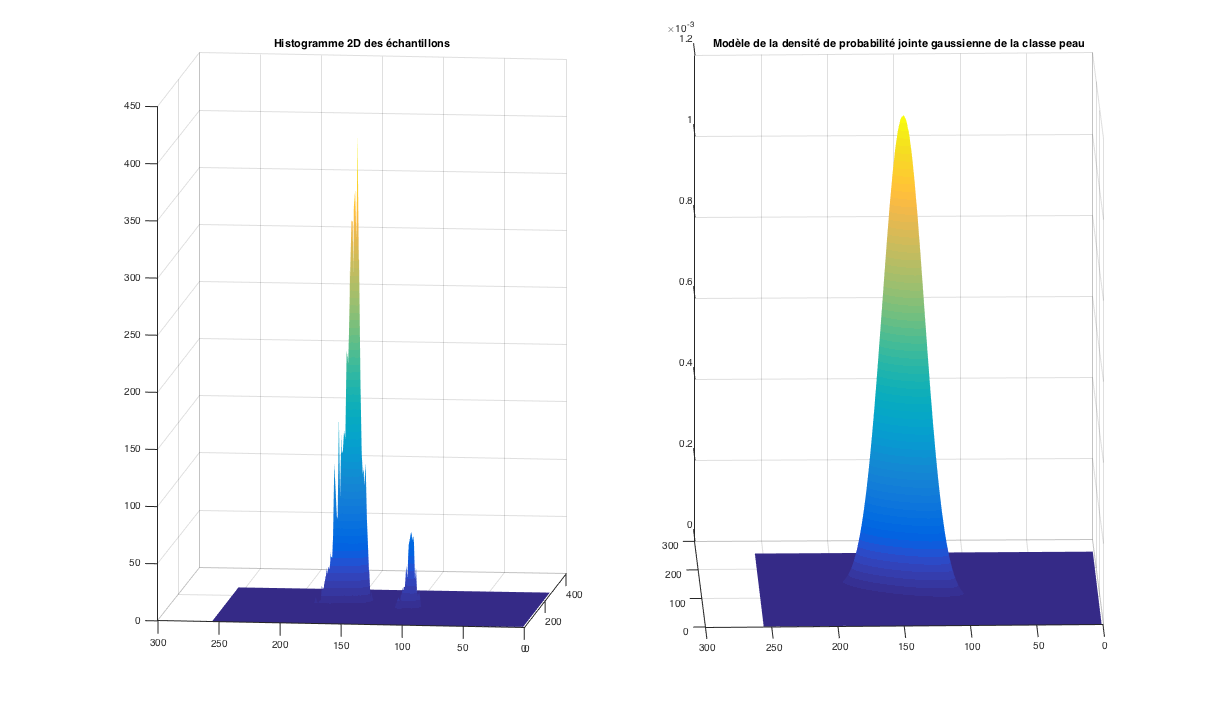
\includegraphics[width=15cm]{exo2_hist2D.png}
\label{fig.exo2_histogramme2D}
\caption{Histogramme 2D des composantes $C_r$ et $C_b$ sur 20 images comparé au modèle gaussien}
\end{figure} 


Comme modèle de probabilité théorique que l'on va utiliser pour modéliser l'information de couleur de la peau on va prendre un modèle \emph{gaussien multi-varié}.

\subsubsection{Calcul des paramètres du modèle}

On rappelle l'équation \ref{eq.gauss.multi} du modèle gaussien multi-varié :
$$
p(\textbf{x}|w_1) = \frac{1}{(2\pi)^{\frac{d}{2}}|\Sigma_1|^{\frac{1}{2}}}\,\text{exp}\left[-\frac{1}{2}(\textbf{x}-\mu_1)^T \Sigma_1^{-1}(\textbf{x}-\mu_1)\right]
$$

\subsection{Partie II : Vers un classifieur bayésien}
\subsubsection{Classe "non-peau"}


\subsubsection{Classifieur optimal}

\newpage
\appendix
\section{Compléments et figures annexes de l'exercice I}
\subsection{Tableau de la probabilité de l'erreur}

On donne dans le tableau ci-dessous les différents résultats que nous donne la classification bayésienne en fonction des paramètres du modèle de la classe 2.
\begin{table}[H]
\center
\begin{tabular}{|c|c|c|c|}
\hline 
$\mu_2$ & $\sigma_2$ & $x_B$ & $\mathbb{P}(\text{erreur})$ \\ 
\hline 
$1$ & $1/ \sqrt{2}$ & $0,5$ & $0,2398$ \\ 
\hline 
$0,5$ & $1/ \sqrt{2}$ & $0,25$ & $0,3818$ \\ 
\hline 
$2$ & $1/ \sqrt{2}$ & $1$ & $0,0787$ \\ 
\hline 
$1$ & $0,25$ & $0,59$ et $1,71$ & $0,0275$ \\ 
\hline 
$1$ & $1$ & $-2,64$ et $0,65$ & $0,3188$ \\ 
\hline 
$1$ & $2$ & $-1,3$ et $1,02$ & $0,2750$ \\ 
\hline 
\end{tabular}
\caption{Probabilité de l'erreur avec de nouveaux paramètres pour la classe 2}

\end{table}


\subsection{Graphiques avec les nouveaux paramètres}
On modifie certains paramètres de la classe 2 et on trace les graphiques correspondant.

\begin{figure}[H]
\center
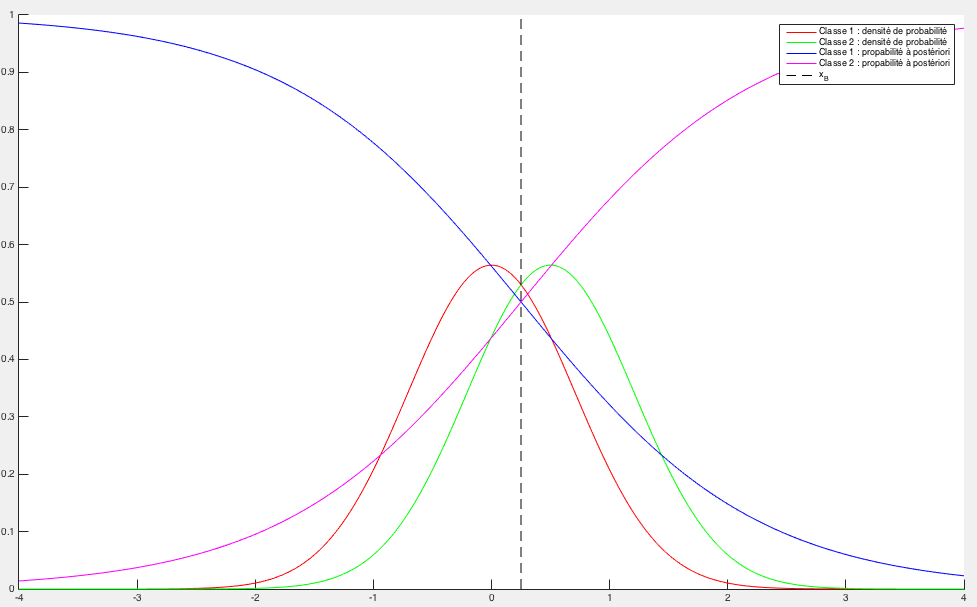
\includegraphics[width=14cm]{exo1_graph_mu05.png}
\caption{Données de probabilités avec $\mu_2 = 0,5$ et $\sigma_2 = 1/\sqrt{2}$}
\end{figure}

\begin{figure}[H]
\center
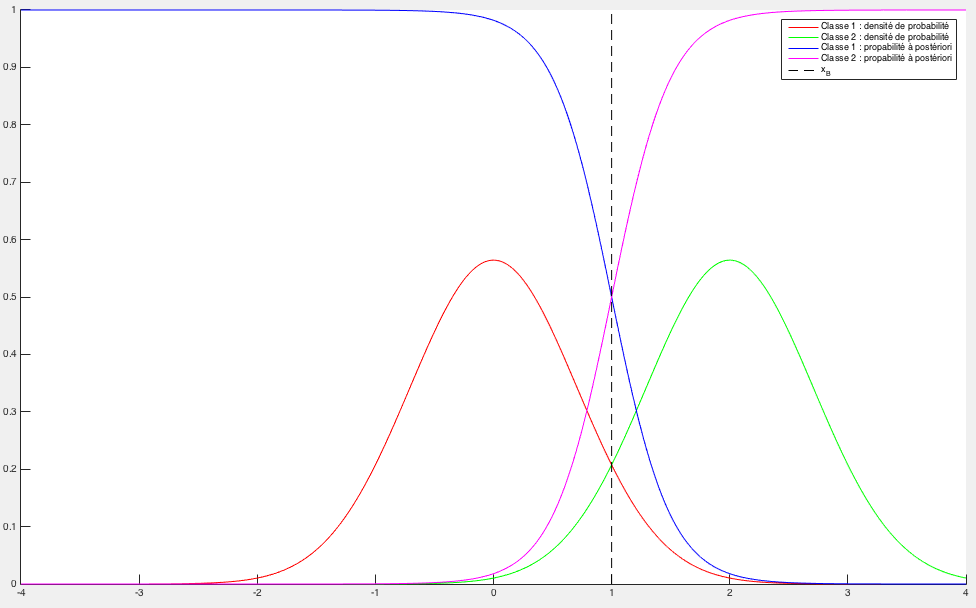
\includegraphics[width=14cm]{exo1_graph_mu2.png}
\caption{Données de probabilités avec $\mu_2 = 2$ et $\sigma_2 = 1/\sqrt{2}$}
\end{figure}

\begin{figure}[H]
\center
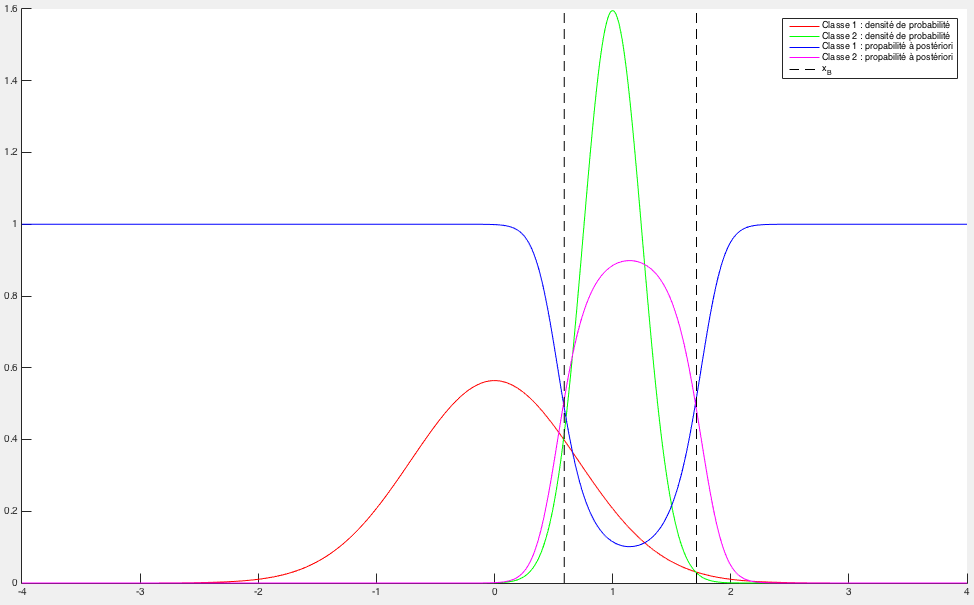
\includegraphics[width=14cm]{exo1_graph_mu1_sigma025.png}
\caption{Données de probabilités avec $\mu_2 = 1$ et $\sigma_2 = 0,25$}
\end{figure}

\begin{figure}[H]
\center
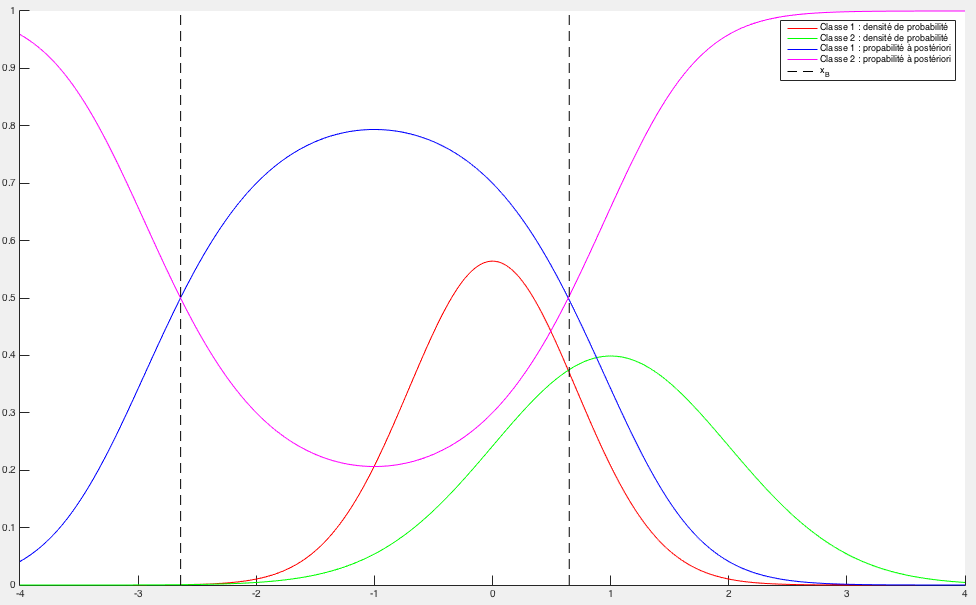
\includegraphics[width=14cm]{exo1_graph_mu1_sigma1.png}
\caption{Données de probabilités avec $\mu_2 = 1$ et $\sigma_2 = 1$}
\end{figure}

\begin{figure}[H]
\center
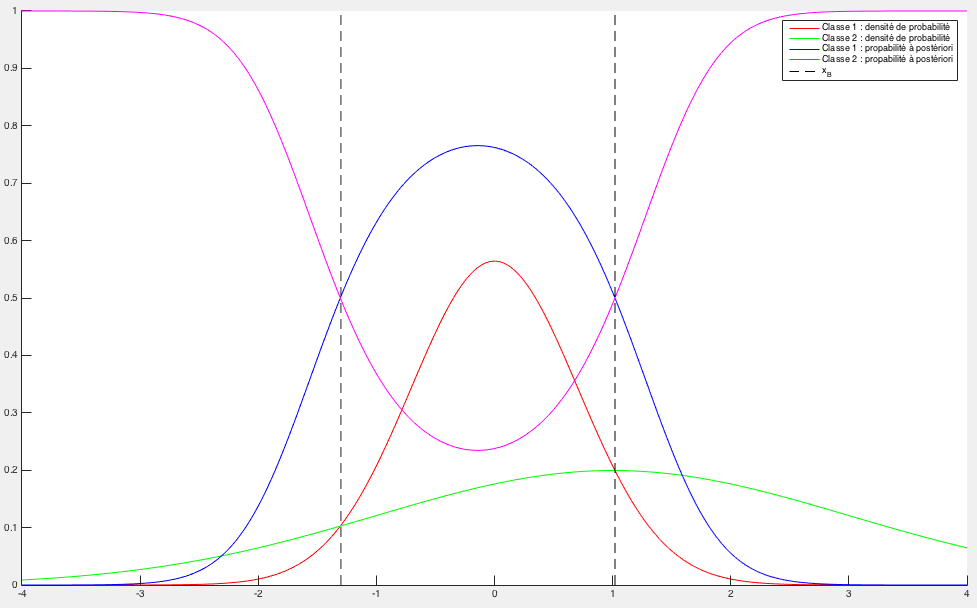
\includegraphics[width=14cm]{exo1_graph_mu1_sigma2.png}
\caption{Données de probabilités avec $\mu_2 = 1$ et $\sigma_2 = 2$}
\end{figure}

\newpage
\section{Code \emph{MatLab} de l'exercice I}

\begin{lstlisting}[language=matlab]
%% TD Reconnaissance de Formes - Exercice 1

clc;
close all;
clear;

Max_x = 4;
Min_x = -4;
Pas = 0.01;
x= [Min_x:Pas:Max_x];
L = length(x);

% Considerons que 2 classes sont modelisees par les densites de
% probabilite gaussiennes suivantes :
pxw1 = exp(-(x.*x))./sqrt(pi);
mu2 = 1;
sigma2 = sqrt(0.5); % ecart-type
%sigma2 = 2;
pxw2 = exp(-(x-mu2).*(x-mu2)/(2*sigma2^2))./sqrt(2*pi*sigma2^2);

%% 1. 1er cas:  Pw1=Pw2=0,5
Pw1 = 0.5;
Pw2 = 1 - Pw1;

px = pxw1 * Pw1 + pxw2 * Pw2; % calcul de la probabilite totale

Pw1x = pxw1 * Pw1 ./ px;
Pw2x = pxw2 * Pw2 ./ px;


% Seuil
i = 1;
g1 = log(pxw1(1) * Pw1);
g2 = log(pxw2(1) * Pw2);
for k = 2 : length(x)
    g1m = log(pxw1(k) * Pw1);
    g2m = log(pxw2(k) * Pw2);
    
    if (g1 - g2)*(g1m - g2m) < 0
        xB(i) = x(k);
        i = i + 1;
    end
    
    g1 = log(pxw1(k) * Pw1);
    g2 = log(pxw2(k) * Pw2);
    
end

% Calcul de l'erreur
%indices = find(x <= xB(1) | xB(2) <= x);
indices = find(x <= xB(1));
M = length(indices);
Perreur = Pas * sum(pxw2(indices) * Pw2);
Perreur = Perreur + Pas * sum(pxw1(indices(M) + 1:L) * Pw1);

%  Traces des densites de probabilites des 2 classes
figure(1)
hold on;
plot(x,pxw1,'color','red');
plot(x,pxw2,'color','green');
plot(x,Pw1x,'color','blue');
plot(x,Pw2x,'color','magenta');
plot([xB(1) xB(1)],[0 1],'--','color','black');
%plot([xB(2) xB(2)],[0 1],'--','color','black');
hold off;
legend('Classe 1 : densite de probabilite','Classe 2 : densite de probabilite', ...
	'Classe 1 : propabilite a posteriori', ...
	'Classe 2 : propabilite a posteriori','x_B');



%% 2. Modification des valeurs de probabilite a priori
Pw1 = 9/10;
Pw2 = 1/10;

px = pxw1 * Pw1 + pxw2 * Pw2; % calcul de la probabilite totale

Pw1x = pxw1 * Pw1 ./ px;
Pw2x = pxw2 * Pw2 ./ px;


% Seuil
i = 1;
g1 = log(pxw1(1) * Pw1);
g2 = log(pxw2(1) * Pw2);
for k = 2 : length(x)
    g1m = log(pxw1(k) * Pw1);
    g2m = log(pxw2(k) * Pw2);
    
    if (g1 - g2)*(g1m - g2m) < 0
        xB(i) = x(k);
        i = i + 1;
    end
    
    g1 = log(pxw1(k) * Pw1);
    g2 = log(pxw2(k) * Pw2);
    
end

% Calcul de l'erreur
indices = find(x <= xB);
M = length(indices);
Perreur = Pas * sum(pxw2(indices) * Pw2);
Perreur = Perreur + Pas * sum(pxw1(indices(M) + 1:L) * Pw1);

%  Traces des densites de probabilites des 2 classes
figure(2) 
hold on
plot(x,pxw1,'color','red');
plot(x,pxw2,'color','green');
plot(x,Pw1x,'color','blue');
plot(x,Pw2x,'color','magenta');
plot([xB xB],[0 1],'--','color','black');
hold off;
legend('Classe 1 : densite de probabilite','Classe 2 : densite de probabilite', ...
	'Classe 1 : propabilite a posteriori', ...
	'Classe 2 : propabilite a posteriori','x_B');

    
% Prise en compte du numerateur uniquement
Pw1x_modif = pxw1 * Pw1;
Pw2x_modif = pxw2 * Pw2;


figure(3) 
hold on
plot(x,pxw1,'color','red');
plot(x,pxw2,'color','green');
plot(x,Pw1x_modif,'color','blue');
plot(x,Pw2x_modif,'color','magenta');
plot([xB xB],[0 0.6],'--','color','black');
hold off;
legend('Classe 1 : densite de probabilite','Classe 2 : densite de probabilite', ...
	'Classe 1 : propabilite a posteriori', ...
	'Classe 2 : propabilite a posteriori','x_B');
\end{lstlisting}

\newpage
\section{Code \emph{MatLab} de l'exercice II}




\end{document}